\section{Ontology construction and entity linking}\label{sec:onto}
\subsection{Ontology construction}
Figure~\ref{fig:owl-design} shows our OWL ontology design, summarizing the main movie-domain classes and their relationships.
\begin{figure}[htbp]
\centering
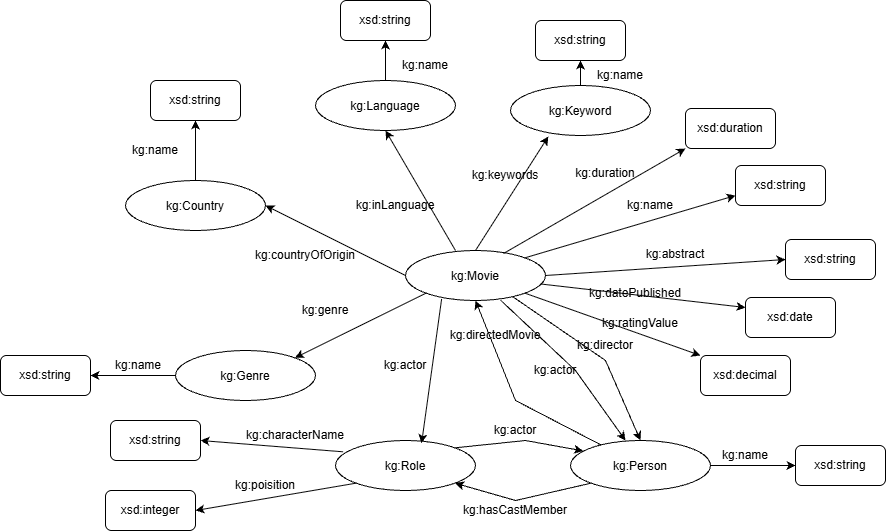
\includegraphics[width=\linewidth,keepaspectratio]{images/ontology.png}
\caption{OWL ontology design for the movie knowledge graph.}
\label{fig:owl-design}
\end{figure}

The ontology defines classes, property domains and ranges, disjoint classes, and cardinality restrictions. Our domain terms use \code{kg:} instead of Schema.org. We do not include broad superclasses such as CreativeWork or Thing.

A movie has at least one name and at most one rating value. An acting role has exactly one actor of type Person, at most one character name, and at most one cast position. These OWL restrictions describe the intended model; missing fields still need separate checks because OWL uses an open-world interpretation.

Two axioms support our reasoning examples. First, \kg{directedMovie} is the inverse of \kg{director}. Second, the path from a director to a directed movie and then to its actors implies \kg{hasCastMember}:
\begin{lstlisting}
kg:directedMovie
  owl:inverseOf kg:director .

kg:hasCastMember
  owl:propertyChainAxiom
    (kg:directedMovie kg:actor) .
\end{lstlisting}
Because actor can point to a person or an acting role, hasCastMember can also point to either. Queries listing actors explicitly select Person resources.


% Figure~\ref{fig:reasoning} illustrates the property chain with example resources.
% The directedMovie edge can first be inferred from a movie's director edge.
% Following it with an actor edge then produces hasCastMember.

% \begin{figure}[t]
% \centering
% \begin{tikzpicture}[
%  n/.style={draw,rounded corners,font=\small,minimum height=7mm},
%  edge/.style={-{Latex},thick},
%  lab/.style={font=\scriptsize,fill=white,inner sep=2pt}]
% \node[n] (director) at (0,0) {Director};
% \node[n] (movie) at (2.3,0) {Movie};
% \node[n] (actor) at (4.6,0) {Actor};
% \draw[edge] (director)--node[lab,above]{directedMovie}(movie);
% \draw[edge] (movie)--node[lab,above]{actor}(actor);
% \draw[edge,dashed] (director.south) to[bend right=35]
%  node[lab,below]{hasCastMember (inferred)} (actor.south);
% \end{tikzpicture}
% \caption{A director-to-actor relationship derived through a movie. Property names use the kg: prefix.}
% \label{fig:reasoning}
% \end{figure}

\subsection{Entity linking}
Movies are matched to Wikidata using their TMDB movie IDs and release years. A matching ID and year allow automatic approval. Weaker candidates require review, while conflicting years can cause rejection. Title matching is used as a fallback. People are matched using TMDB person IDs, human type, and normalized names. Name and filmography searches provide fallback candidates.

Countries and languages are matched by ISO codes. Genres are matched using film-genre names and linked with \code{skos:closeMatch}, since the genre categories may not have exactly the same meaning. Movies, people, countries, and languages use \code{owl:sameAs} for approved identity matches.

The scripts save candidate evidence in CSV files and approved links in separate Turtle files. The current outputs contain 198 movie links, 1,591 person links, and 112 lookup links. DBpedia URIs are constructed from English Wikipedia titles returned by Wikidata; they have not been independently checked against DBpedia. Automatic approval therefore does not guarantee that every link is correct.
